\documentclass[12pt]{article}

% Ћирилица: кодирање фонта и језик (српски, ћирилица)
\usepackage[T2A]{fontenc}
\usepackage[utf8]{inputenc}
\usepackage[serbianc]{babel}

% Величина стране и маргине
\usepackage[a4paper,top=2cm,bottom=2cm,left=2.5cm,right=2.5cm]{geometry}

% Корисни пакети
\usepackage{amsmath}
\usepackage{enumitem}
\usepackage{float}
\usepackage{booktabs}
\usepackage{tcolorbox}
\tcbuselibrary{breakable}
\usepackage[colorlinks=true, allcolors=blue]{hyperref}

% Цртање електричних кола (европски симболи)
\usepackage[european]{circuitikz}
\usetikzlibrary{babel}

% Оквир за решене примере
\newtcolorbox[auto counter]{primer}{breakable,
    colback=white, colframe=black!55, colbacktitle=black!55, coltitle=white,
    fonttitle=\bfseries\small, title={Пример~\thetcbcounter},
    boxrule=0.5pt, arc=1.5pt, left=6pt, right=6pt, top=3pt, bottom=3pt,
    before skip=8pt, after skip=10pt}

% Оквир за кључне формуле
\newtcolorbox{kljucno}{colback=blue!4, colframe=blue!45!black,
    boxrule=0.5pt, arc=1.5pt, left=8pt, right=8pt, top=4pt, bottom=4pt}

\title{KE - Jetronic систем убризгавања - пропитивање}
\author{Аутоелектронски системи 2}
\date{}

\begin{document}
\maketitle

\section{KE-Jetronic систем убризгавања} 

Мора да се зна да се означи која компонента је где. 

\begin{figure}[H]
    \centering
    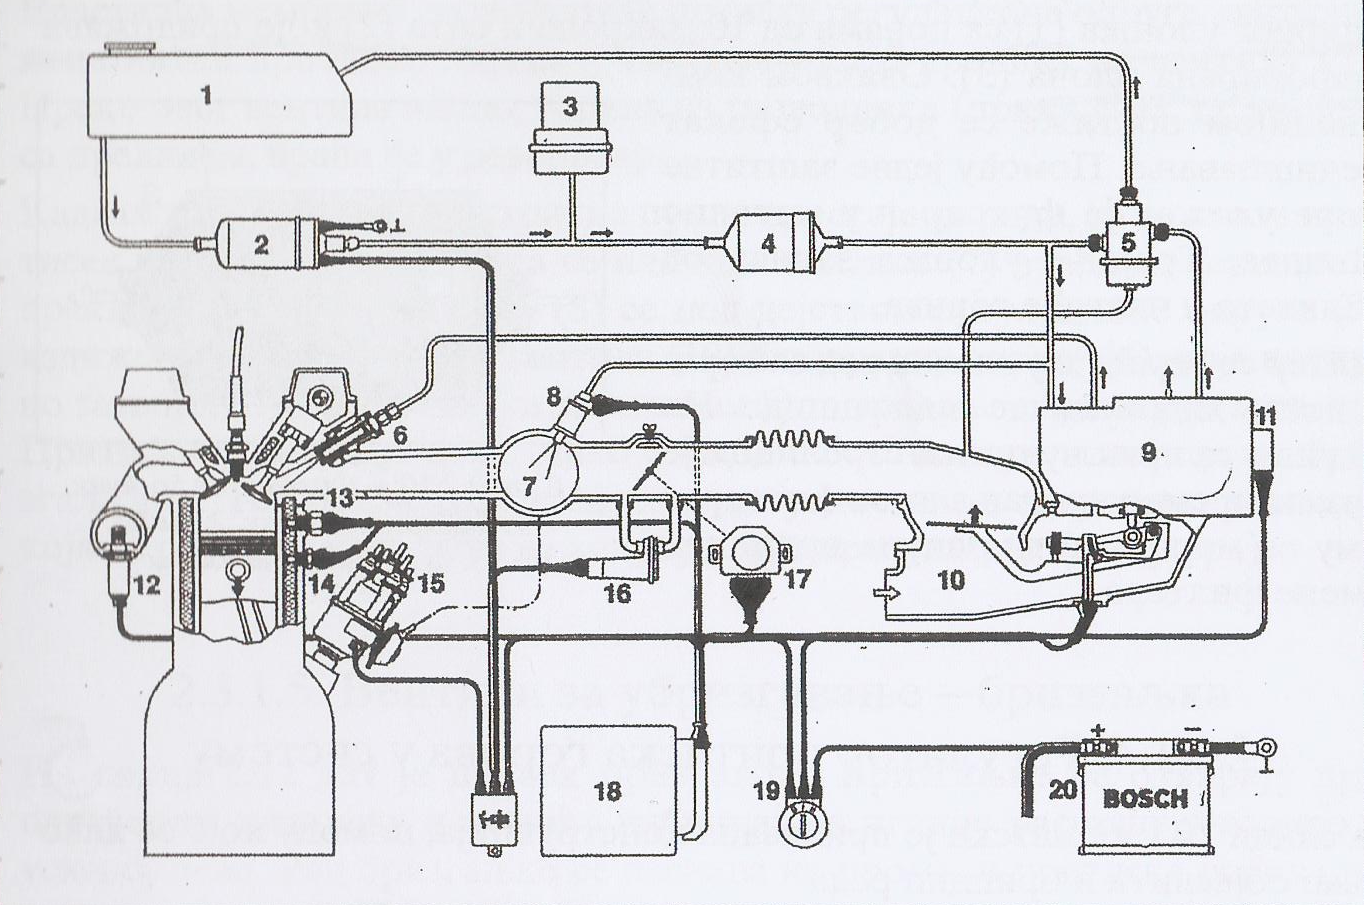
\includegraphics[width=0.9\textwidth]{slike/KEe.png}
    \caption{Основна шема KE Jetronic система убризгавања}
    \label{fig:primer}
\end{figure}

\begin{kljucno}
\begin{enumerate}
    \item[1.] Резервоар за гориво - место са бензином
    \item[2.] Електрична пумпа за гориво - усисавање бензина
    \item[3.] Хидраулична пригушница за гориво - регулација константног притиска
    \item[4.] Филтер за гориво 
    \item[5.] Регулатор системског притиска - одржавање притиска
    \item[6.] Бризгаљка 
    \item[7.] Усисни колектор 
    \item[8.] Бризгаљка за хладан старт
    \item[9.] Дозатор - Комора за дозирање бризгаљки
    \item[10.] Мерач протока ваздуха (протокомер)
    \item[11.] Електро-хидраулични регулатор (актуатор)
    \item[12.] ЛАМБДА сонда - сензор мешавине
    \item[13.] Временски термо-прекидач 
    \item[14.] Сензор температуре мотора
    \item[15.] Разводник паљења 
    \item[16.] Регулатор празног хода
    \item[17.] Потенциометар пригушног лептира
    \item[18.] Електронска управљачка јединица
    \item[19.] Контакт-кључ
    \item[20.] Акумулатор
\end{enumerate}
\end{kljucno}

\subsection{Дозатор}

Компонента која сачињава дозатор је \textbf{разводник количине горива}

Разводник дозира гориво и разводи га до бризгаљки, према количини усисаног
ваздуха. Померај мерне плоче преноси се на регулациони клип. Што се клип више
подигне, већи је отвор регулационих прореза (по један за сваки цилиндар) и кроз
њих протиче више горива. Веза између отклона мерне плоче и отвора прореза је
линеарна.

Са друге стране на клип делује притисак горива, који уравнотежује силу ваздуха
на мерну плочу, па клип тачно прати кретање плоче. Зато системски притисак мора
бити тачно регулисан, јер свака његова промена директно мења $\lambda$. Када се
мотор угаси, клип се спусти на заптивни прстен и спречава одлив горива.

\begin{figure}[H]
    \centering
    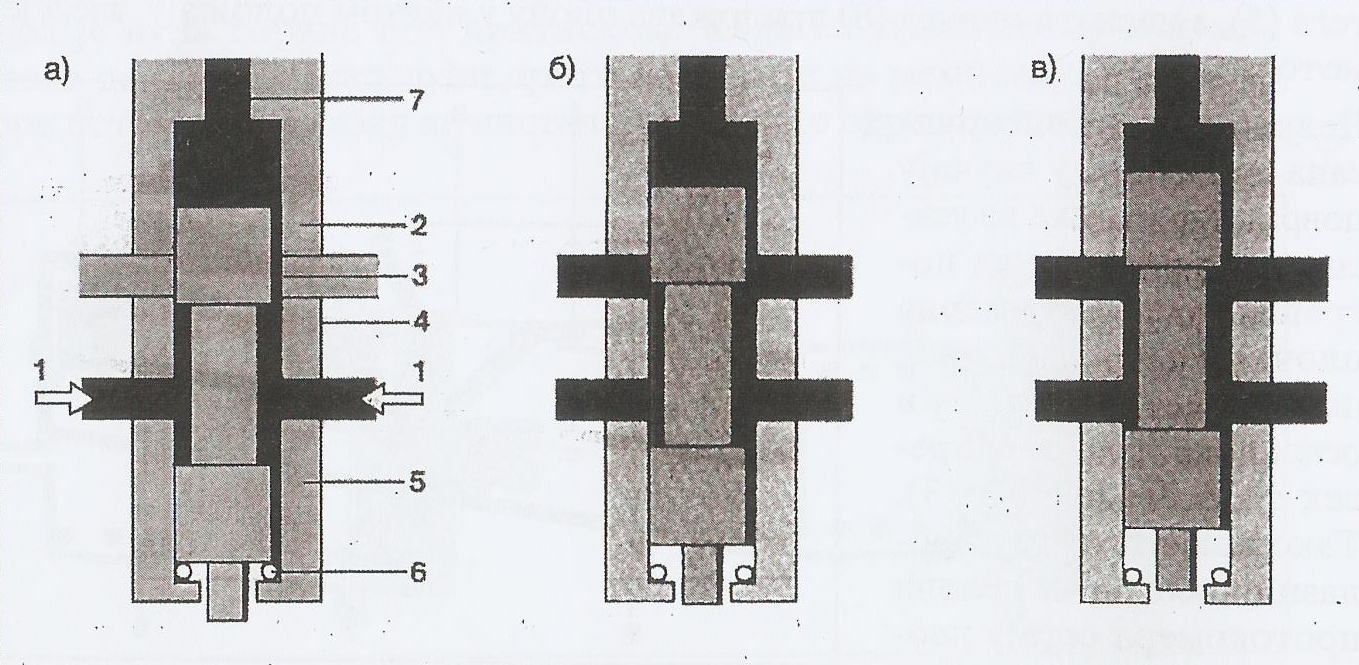
\includegraphics[width=0.7\textwidth]{slike/KEe4.png}
    \caption{Разводник количине горива}
    \label{fig:primer}
\end{figure}

\subsection{Електрохидраулични регулатор (актуатор)}

Актуатор, према електричним импулсима из управљачке јединице, мења притисак у
доњим коморама вентила диференцијалног притиска. Тако се убризгана количина
горива коригује много брже и прецизније, у зависности од режима рада мотора.

Уграђен је на дозер. Гориво под системским притиском пролази кроз
млазницу, испред које је одбојна плоча [11. ] спојена са котвом електромагнета. Струја
кроз намотаје електромагнета, заједно са сталним магнетом, ствара обртни момент
на котви који је сразмеран јачини струје. Тиме се подешава положај одбојне
плоче, а самим тим и пад притиска горива између улаза и излаза регулатора.
Промена притиска у доњим коморама преноси се на горње и мења количину горива
према бризгаљкама.

\begin{figure}[H]
    \centering
    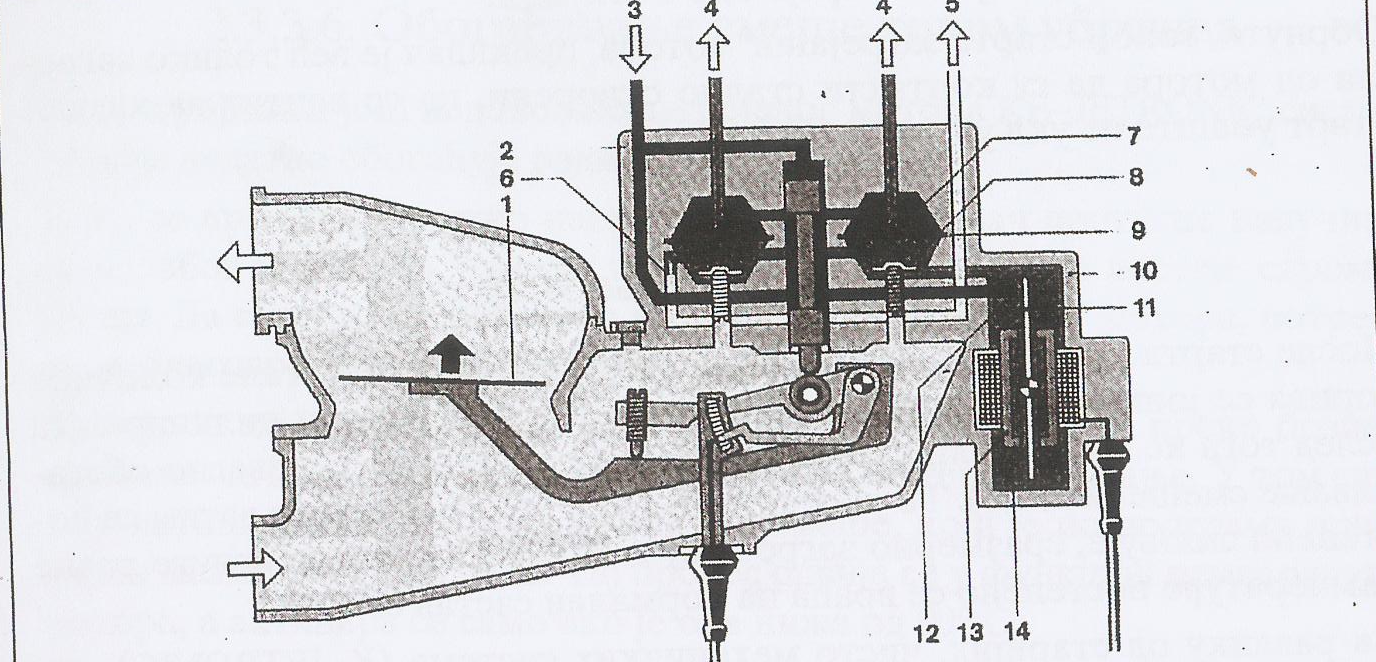
\includegraphics[width=0.6\textwidth]{slike/KE6e.png}
    \caption{Формирање смеше}
    \label{fig:primer}
\end{figure}

Због мале инерције покретних делова регулатор реагује веома брзо. Ако се
промени смер струје, плоча се одмакне од млазнице и бризгаљке потпуно престају
да добијају гориво, што се користи код кочења мотором и ограничења броја
обртаја. Ако нестане струје (квар), регулатор је механички подешен да одржава
$\lambda = 1$, па се возилом може доћи до сервиса.

\section{Режими рада КЕ мотора}

Потребно је знати ову поделу:

\begin{itemize}[itemsep=0pt]
    \item хладан старт,
    \item загревање мотора,
    \item обогаћивање смеше током убрзања,
    \item обогаћивање смеше при пуном оптерећењу,
    \item празан ход хладног мотора,
    \item празан ход.
\end{itemize}

Али додатно и:

\subsection{Празан ход}

Биметални вентил не прати стварни број обртаја, већ додаје ваздух само према
температури. Зато се са старењем мотора број обртаја у празном ходу
непотребно повећава, а са њим и потрошња.

\textbf{Регулатор празног хода} то решава. Током целог рада одржава стабилан и
што мањи број обртаја, без обзира на оптерећење и старење мотора. Налази се
у заобилазном воду. Управљачка јединица упоређује стварни број обртаја са
програмираним (који зависи од температуре мотора). Ако се разликују,
регулатор отвара или притвара заобилазни вод док се не постигне жељена
вредност. Регулатор ради као обртни магнет: окреће плочу за око $60^\circ$ и
тако отвара или затвара канал.

\begin{figure}[H]
    \centering
    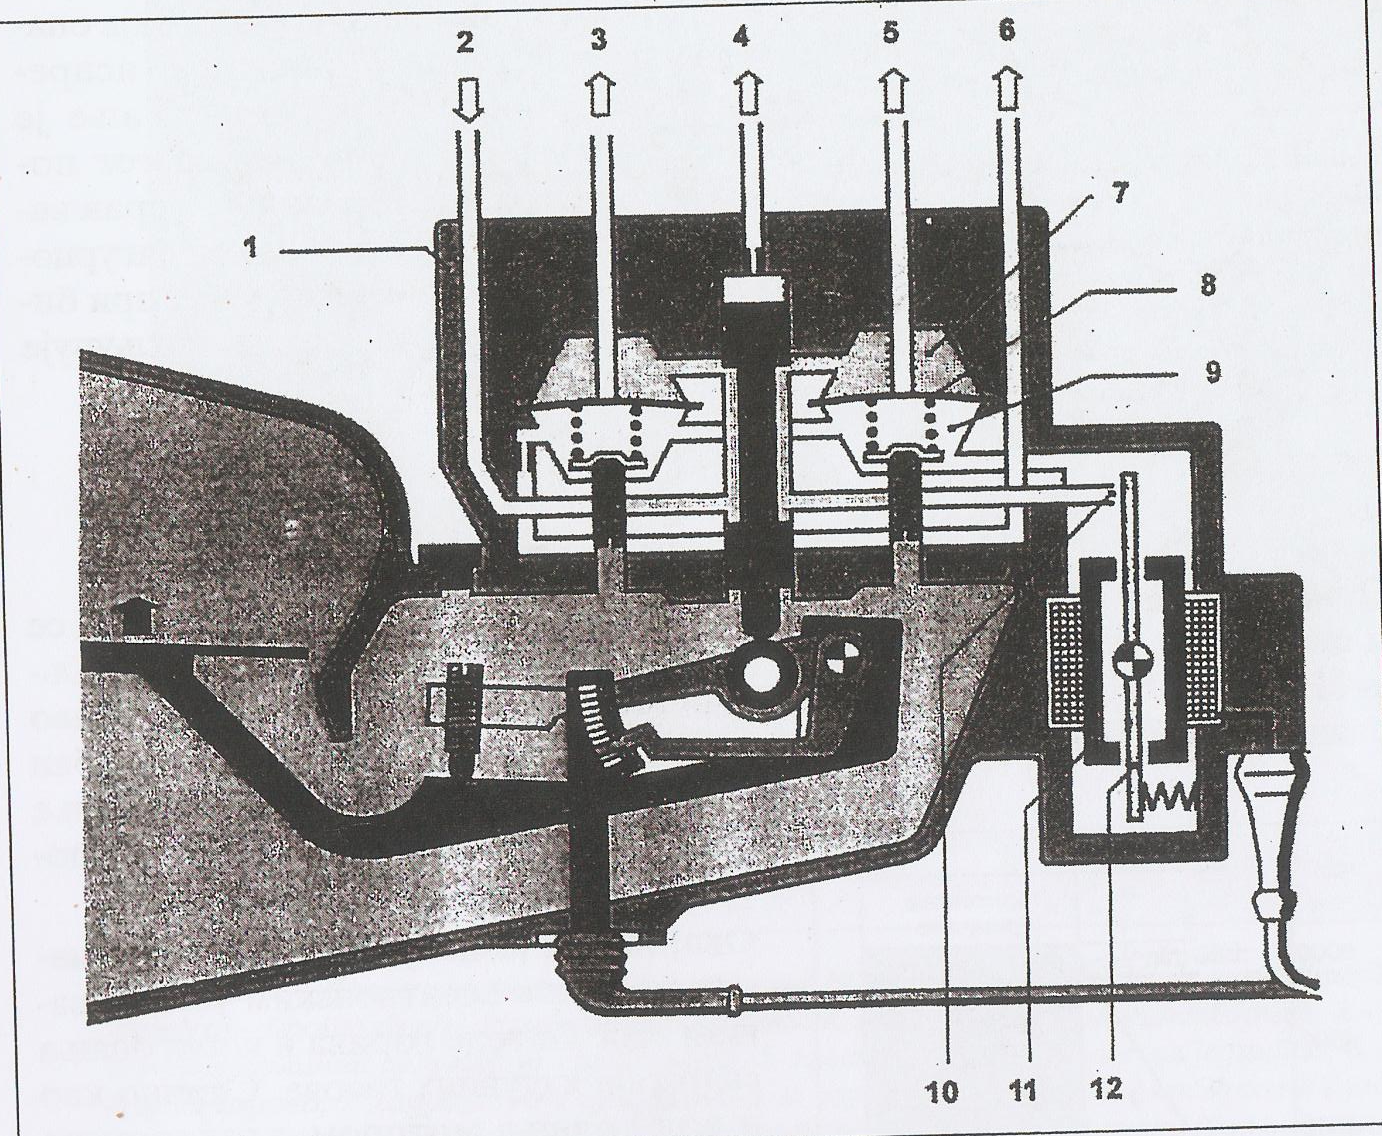
\includegraphics[width=0.4\textwidth]{slike/KEe7.png}
    \caption{Регулатор празног хода}
    \label{fig:primer}
\end{figure}


\section{Управљаче функције}

Управљачка јединица на овај начин делује у следећим случајевима:
\begin{itemize}[itemsep=0pt]
    \item кочење мотором,
    \item ограничење броја обртаја,
    \item висинска корекција смеше,
    \item ЛАМБДА регулација.
\end{itemize}

\section{Електрична шема система}

\begin{figure}[H]
    \centering
    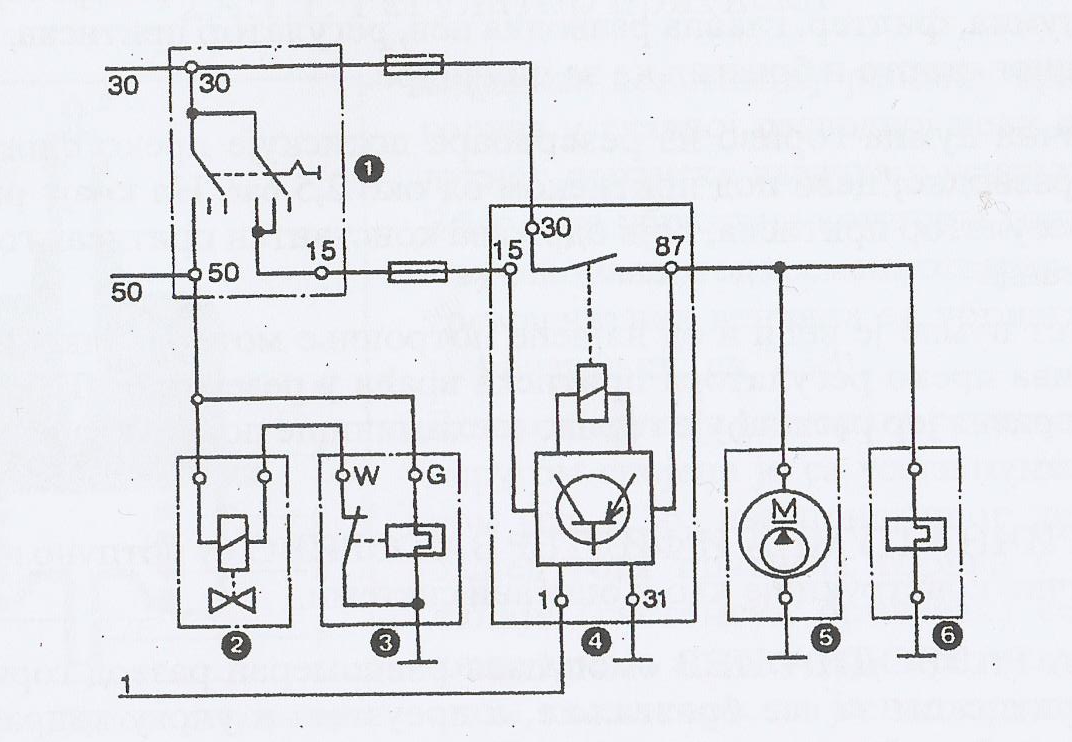
\includegraphics[width=0.9\textwidth]{slike/KEe-sis.png}
    \caption{}
    \label{fig:primer}
\end{figure}


\end{document}